\appendix

\chapter{Literaturrecherche}
\label{sec:appendix_literature_research}

Dieser Anhand enthält zusätzliche Materialien zur durchgeführten Literaturrecherche. \autoref{tab:appendix_search_filter} enthält die genauen Konfiguration der Suchen für die einzelnen Datenbanken und \autoref{fig:appendix_literature_research_results} die Anzahl der Ergebnisse pro Datenbank.

Eine Übersicht über die Kontexte, in welchen die resultierenden Arbeiten Erklärungen analyisert haben, ist in \autoref{fig:appendix_literature_research_results} zu finden.

\begin{table}[htb!]
    \centering
    \begin{tabular}{p{0.3\textwidth}p{0.64\textwidth}}
        \hline
        Datenbank           & Aktivierte Filter \\
        \toprule
        ACM Digital Library & Content-Type: PDF \\
        \tablerowspacing
        IEEE Xplore         & Type: [Conferences, Journals] \\
                            & Subscribed Content Only \\
        \tablerowspacing
        Science Direct      & Article Type: [Research Articles, Book chapters] \\
                            & Subject Area: Computer Science \\
        \tablerowspacing
        Springer Link       & Discipline: Computer Science \\
        \toprule
    \end{tabular}
    \caption{Zusätzliche Filter bei der Literaturrecherche in den Datenbanken}
    \label{tab:appendix_search_filter}
\end{table}

\begin{figure}[htb!]
    \centering
    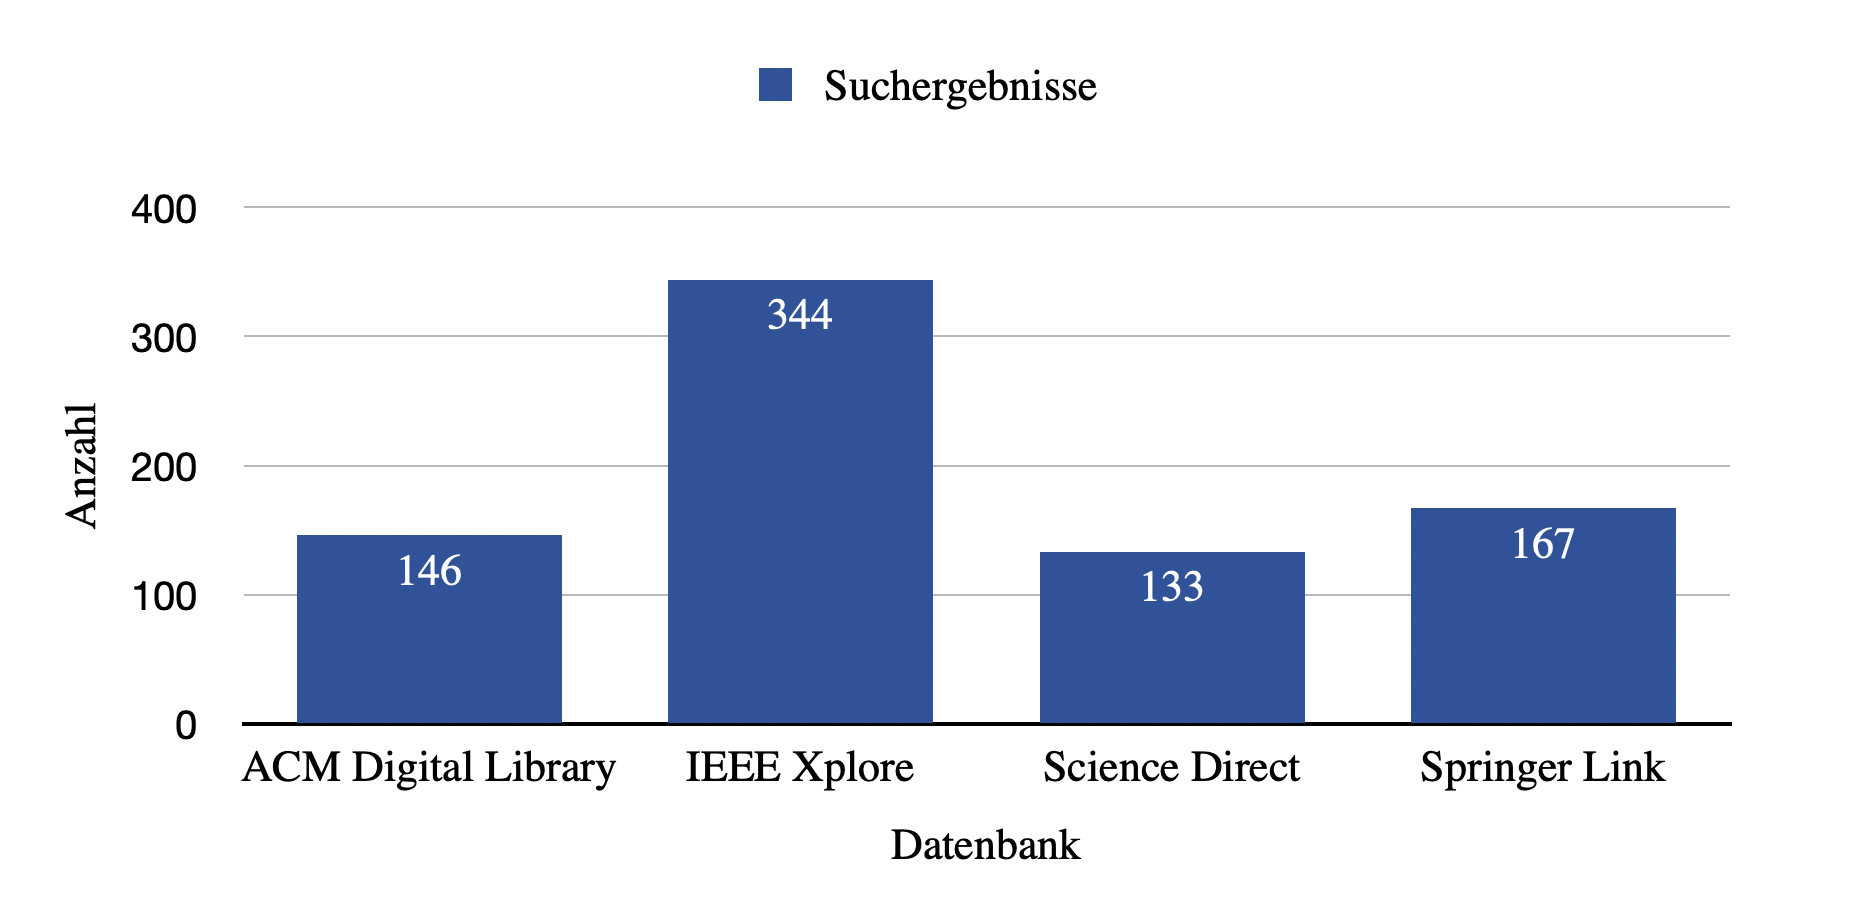
\includegraphics[width=0.75\textwidth]{contents/04_literature_review/res/database_results.png}
    \caption{Anzahl der Suchergebnisse in der Literaturrecherche pro Datenbank}
    \label{fig:appendix_literature_research_results}
\end{figure}

\newpage

\begin{table}[htb!]
    \begin{center}
        \begin{tabular}{p{.3\textwidth}p{.64\textwidth}}
            \hline
            Kontext                   & Quellen \\
            \toprule
            Allgemein                           &
                \cite{chazette_end-users_nodate} \cite{chazette2020explainability} \cite{chazette_knowledge_nodate} \cite{eiband_impact_2019} \cite{kohl_explainability_2019} \cite{ribera2019can} \cite{lim_2009_assessing} \\
            \tablerowspacing
            Intelligente Systeme (z.B. XAI)      & 
                \cite{waa_evaluating_2021} \cite{mucha_interfaces_2021} \cite{sokol_explainability_2020}  \cite{abdulrahman_belief-based_2019} \cite{brennen_what_2020} \cite{schaffer_i_2019} \cite{weitz_you_2019} \cite{riveiro_thats_2021} \cite{martin_developing_2019} \cite{martin_evaluating_2021} \cite{rosenfeld_explainability_2019} \cite{cassens_ambient_2019} \cite{cirqueira_scenario-based_2020}  \cite{ehsan_human-centered_2020} \cite{rjoob_towards_2021} \cite{thomson_knowledge--information_2020} \cite{chari_explanation_2020} \cite{sokol_one_2020}  \cite{neerincx_using_2018} \cite{schrills_color_2020} \cite{sovrano_modelling_2020} \cite{gunning2019darpa} \cite{doshi2017towards} \cite{cheng2019explaining}\\
            \tablerowspacing
            Empfehlungssysteme                  & 
                \cite{tintarev_designing_nodate} \cite{sato_context_nodate} \cite{balog_measuring_2020}  \cite{kouki_user_2017} \cite{tsai_evaluating_2019} \cite{hernandez-bocanegra_effects_2020} \cite{kunkel_let_2019} \cite{tintarev2015explaining} \cite{sato_action-triggering_2019} \cite{tsai_effects_2020} \cite{nunes_systematic_2017} \cite{tintarev2007survey}
            \\
            \tablerowspacing
            Autonomes Fahren                    &
                \cite{wiegand_id_2020} \cite{haspiel_explanations_2018} \cite{koo_understanding_2016} \cite{koo_why_2015} \cite{wiegand2019drive} \cite{du2019look}
            \\
            \tablerowspacing
            Mensch-Roboter-Interaktion          &
                \cite{stange_effects_2021} \cite{kaptein_personalised_2017} \cite{zolotas_towards_2019} \cite{wang_is_2018} \cite{zhu_effects_2020}
            \\
            \tablerowspacing
            Spezifische Domänen                 &
                \cite{yamada_evaluating_2016} \cite{zahedi_towards_2019}
            \\
            \toprule
        \end{tabular}
    \end{center}
    \caption{Kontexte von erklärbaren Systemen, die von in der Literaturrecherche betrachteten Arbeiten untersucht wurde}
\end{table}

\newpage

\chapter{Integration von Erklärungen}

In diesem Anhang sind zusätzliche Informationen zur Integration von Erklärungen in \textit{NUNAV Navigation} enthalten.

\begin{table}[htb!]
    \begin{tabular}{p{.25\textwidth}p{.56\textwidth}p{.1\textwidth}}
        \hline
        Thema & Beschreibung        & Anzahl \\
        \toprule
        Feature Request             & Im Review werden neue Funktionen gefordert. & 18 \\
        \tablerowspacing
        Kollaboratives Routing      & Das Review deutet auf ein fehlendes Verständnis, was der Grundgedanke des
                                        kollaborativen Routings ist, hin. & 16 \\
        \tablerowspacing
        Schlechte Route             & Das Review enthält eine Beschwerde über eine bestimmte Routenführung. & 9 \\
        \tablerowspacing
        GPS-Verständnis             & Das Review deutet auf ein fehlendes Verständnis für schlechten GPS-Empfang hin. & 3 \\
        \tablerowspacing
        Offline-Modus-Verständnis   & Das Review deutet auf ein fehlendes Verständnis der Offline-Karten-Funktion 
                                        hin. & 3 \\
        \tablerowspacing
        Fehlende Information        & Das Review enthält eine Forderung nach mehr Informationen,
                                        die in NUNAV angezeigt werden sollen. & 3 \\
        \tablerowspacing
        Schlechte Suchergebnisse    & Im Review wird die Qualität der Suchergebnisse bemängelt. & 3 \\
        \tablerowspacing
        Verständnis Routenfarbe     & Im Review werden Nachfragen zur Einfärbung der Route gestellt. & 2 \\
        \tablerowspacing
        Falsche Kartendaten         & Im Review werden falsche Kartendaten bemängelt. & 1 \\
        \toprule
    \end{tabular}
    \label{tab:appendix_review_subjects}
    \caption{Anzahl der Reviews im Google Play Store und Apple App Store mit mehrfach vorkommenden Themen}
\end{table}

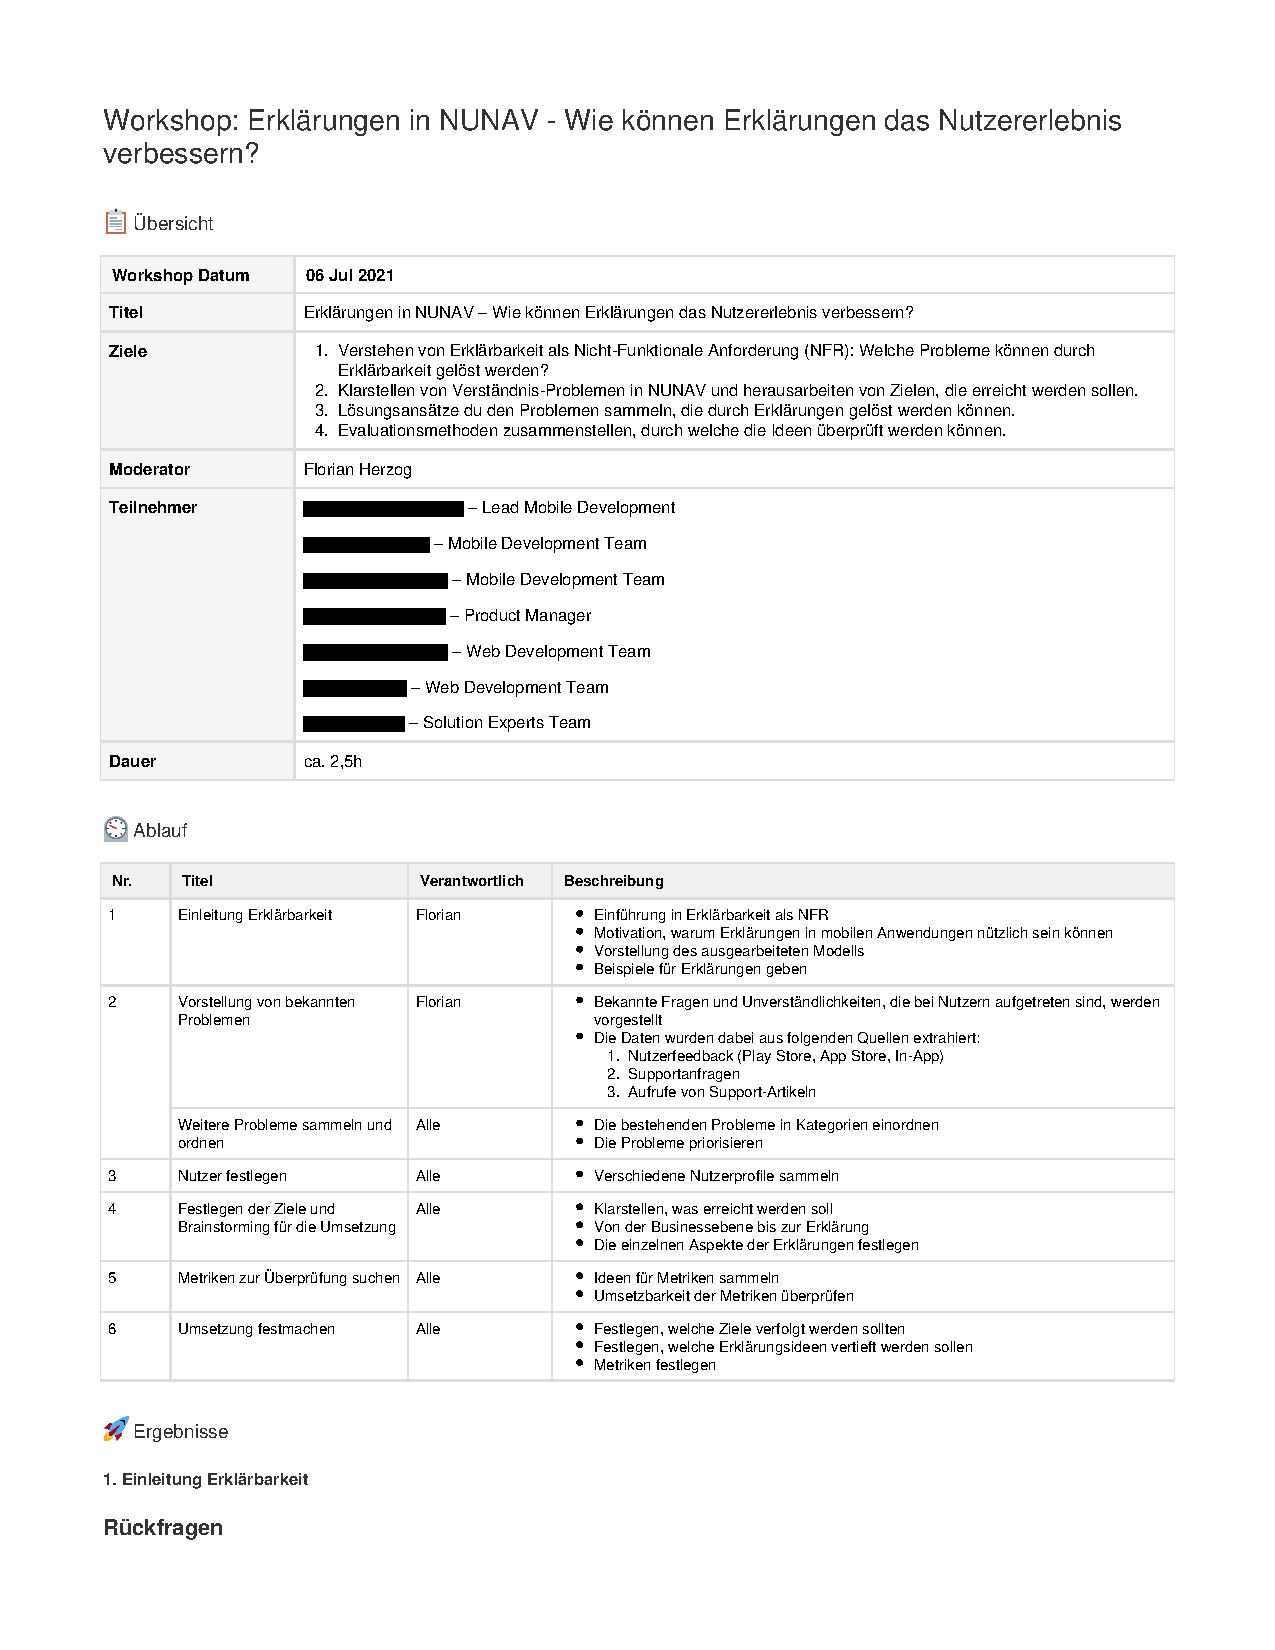
\includepdf[pages=1, scale=0.85,frame, pagecommand=\section*{Workshop zur Integration von Erklärungen}\label{sec:appendix_workshop_protocol}]{contents/a_appendix/res/workshop.pdf}
\includepdf[pages=2-, scale=0.85,frame]{contents/a_appendix/res/workshop.pdf}

\section*{Hife-Center-Artikel: Collaborative Routing}
\label{sec:help_center_collaboratrive_routing}

Wir geben jedem Nutzer eine individuelle Route, um an sein Ziel zu kommen. Diese Route steht immer in Abhängigkeit zu allen anderen Nutzern und sorgt dafür, dass alle Fahrzeuge bestmöglich auf die bestehende Infrastruktur verteilt werden. Durch diese Schwarmintelligenz sind Routingmodelle möglich, die weit über das herkömmliche \glqq Kürzester Weg\grqq{}-Modell hinausgehen und so Staus aktiv vermeiden. 

\smallskip

\noindent Man nennt diese Art des Routings "Collaborative Routing". 

\section*{Hife-Center-Artikel: Routeneinflüsse}
\label{sec:help_center_routing_data}

\noindent Jede berechnete Route entstammt dem neuartigen Ansatz des Collaborative Routings. Dabei werden eine Vielzahl von Variablen berücksichtigt:

\begin{itemize}
    \item Die Routen von NUNAV-Nutzern in Ihrer Nähe
    \item Sperrungen
    \item Baustellen
    \item Aktuelle Verkehrsverzögerungen
    \item und viele mehr....
\end{itemize}

\noindent Anders als bei herkömmlichen Navigationssystemen ist eine \textbf{NUNAV-Route} keinesfalls statisch. Aufgrund der dynamischen Veränderung des Verkehrs berechnen wir Ihnen mehrfach in der Minute Ihre aktuell schnellste individuelle Route unter Berücksichtigung der aktuellen Verkehrslage.

\smallskip

\noindent Das führt dazu, dass \textbf{NUNAV-Route} intelligent und stauvermeidend auf das vorhandene Straßennetz verteilt werden.

\smallskip

\noindent Bei alternativen Navigationssystemen wird meistens egoistisch gehandelt, es oft geht darum, deren Nutzer auf dem kürzesten Wege zu seinem Ziel zu bringen. Dieser Ansatz ist keineswegs stauvermeidend, sondern verursacht oft das Gegenteil.

\smallskip

\noindent Bei NUNAV hingegen, sind Sie Teil einer Gemeinschaft, welche alle Nutzer schnellstmöglich und stauvermeidend an Ihr Ziel bringt. Die wichtigsten Vorteile von \textbf{NUNAV-Route} lauten daher wie folgt:

\begin{itemize}
    \item Stauvermeidend durch den Ansatz des Collaborative Routings
    \item CO2 Einsparung durch weniger Stau und Fahrtzeit
    \item Gemeinschaftliches Handeln führt zu einer Verbesserung der generellen Verkehrslage
\end{itemize}

\noindent Je mehr Nutzer, sich mit \textbf{NUNAV-Route} zu Ihrem Ziel navigieren lassen, desto größer ist der Effekt, den wir gemeinsam erzielen können. Aus diesem Grund würden wir uns freuen, wenn Sie uns an Ihre Freunde und Familien weiterempfehlen.

\smallskip

\noindent Wir hoffen, dass wir Ihnen mit diesem Artikel die Entstehung Ihrer individuellen \textbf{NUNAV-Route} etwas näher bringen konnten.

\newpage

\section*{Prototypen der Erklärung zum aktuellen Verkehrsaufkommen}
\label{sec:appendix_traffic_volume}

\begin{figure}[htb!]
    \centering
    \subfloat[1. Prototyp zur Darstellung des aktuellen Verkehrsaufkommens]
    {
        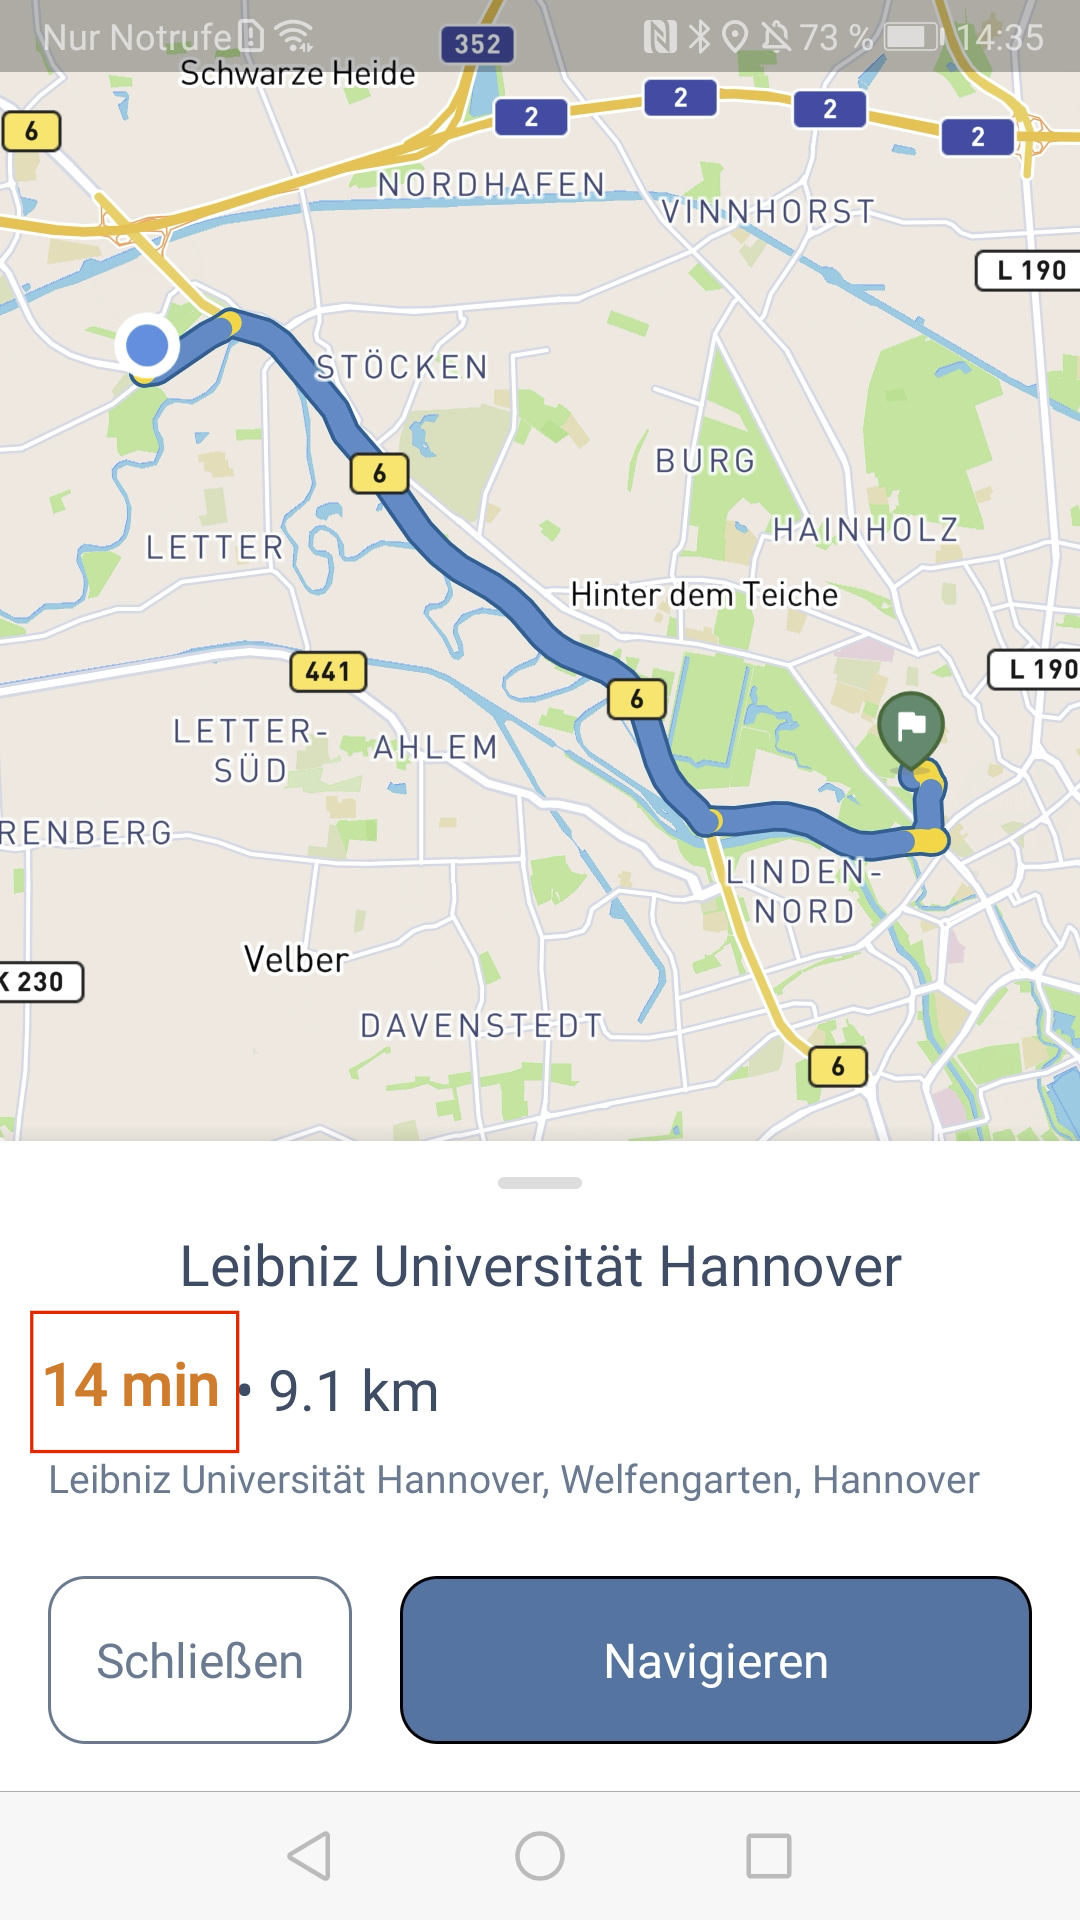
\includegraphics[width=.27\textwidth]{contents/06_model_evaluation/01_integration/res/03_traffic_volume/prototype_11.png}
    }
    \hspace{.055\textwidth}
    \subfloat[2. Prototyp zur Darstellung des aktuellen Verkehrsaufkommens]
    {
        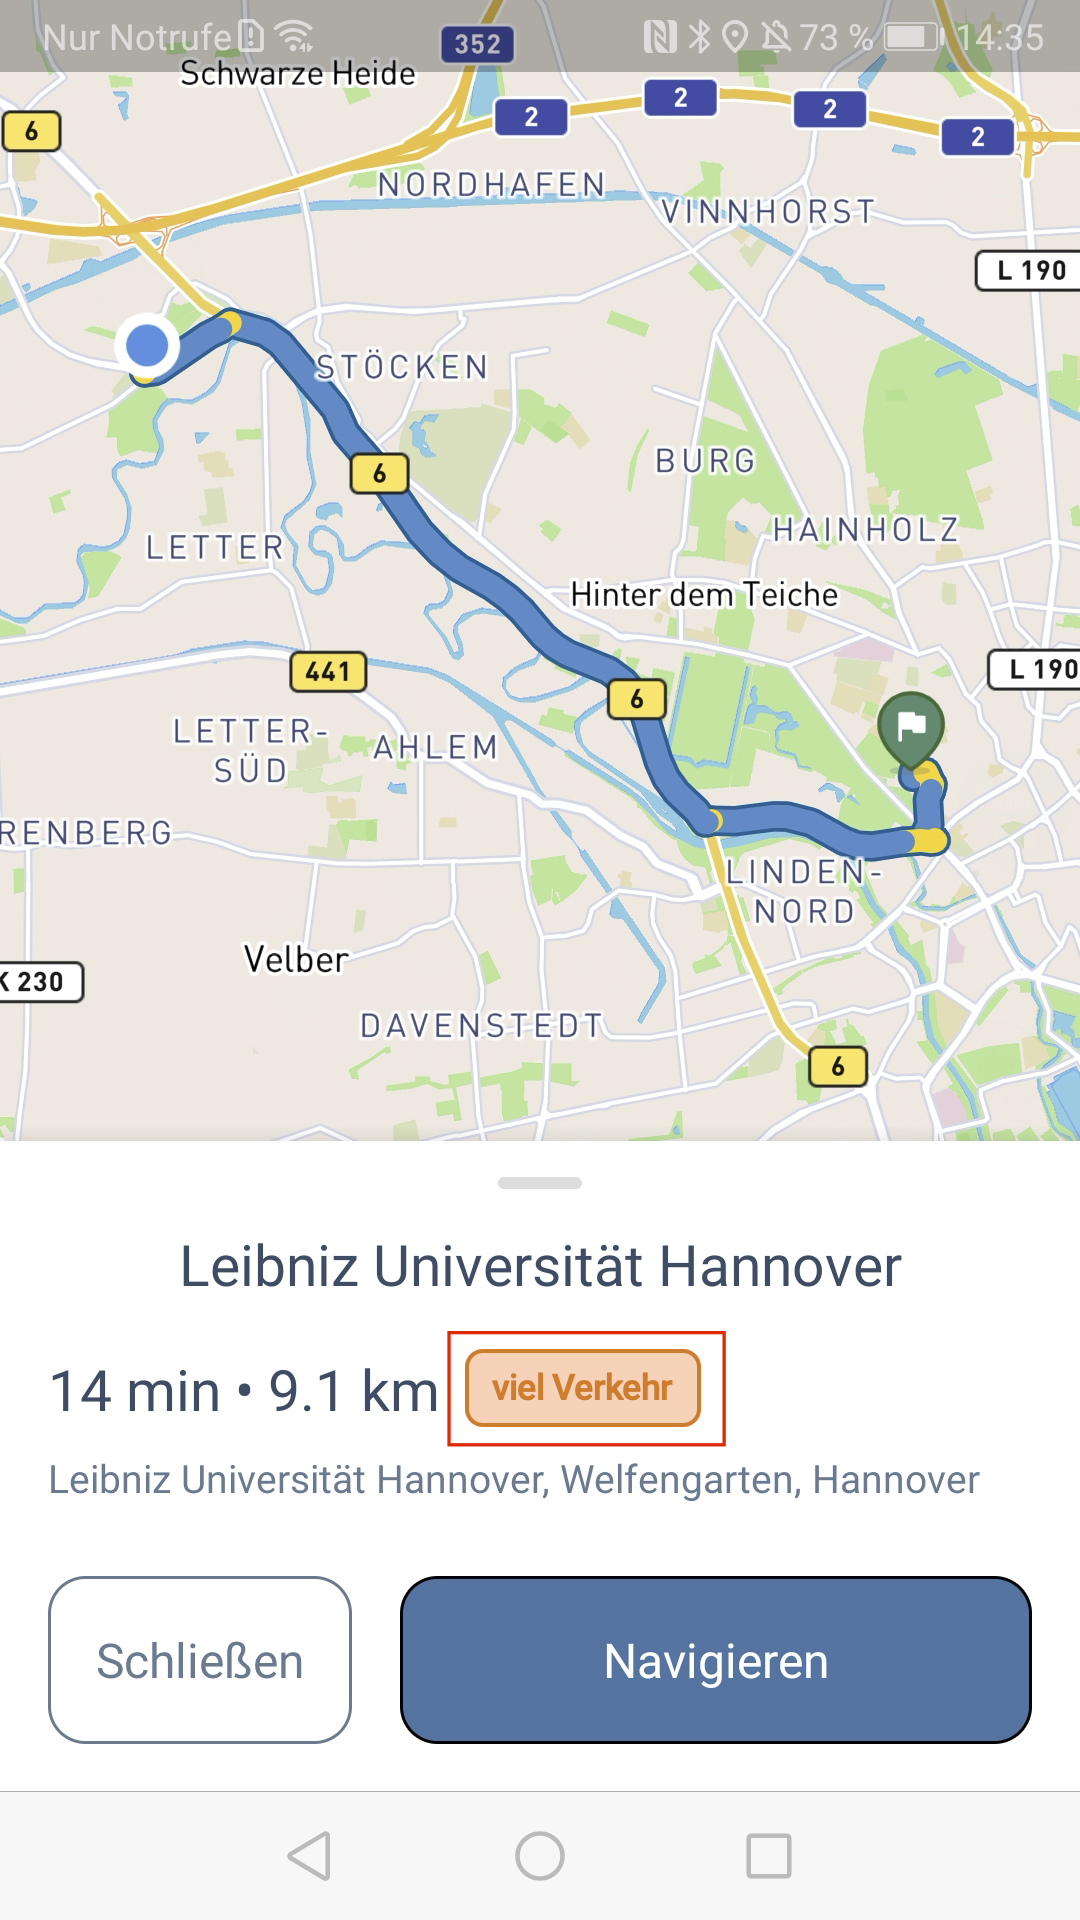
\includegraphics[width=.27\textwidth]{contents/06_model_evaluation/01_integration/res/03_traffic_volume/prototype_12.png}
    }
    \hspace{.055\textwidth}
    \subfloat[Finales Design zur Darstellung des aktuellen Verkehrsaufkommens]
    {
        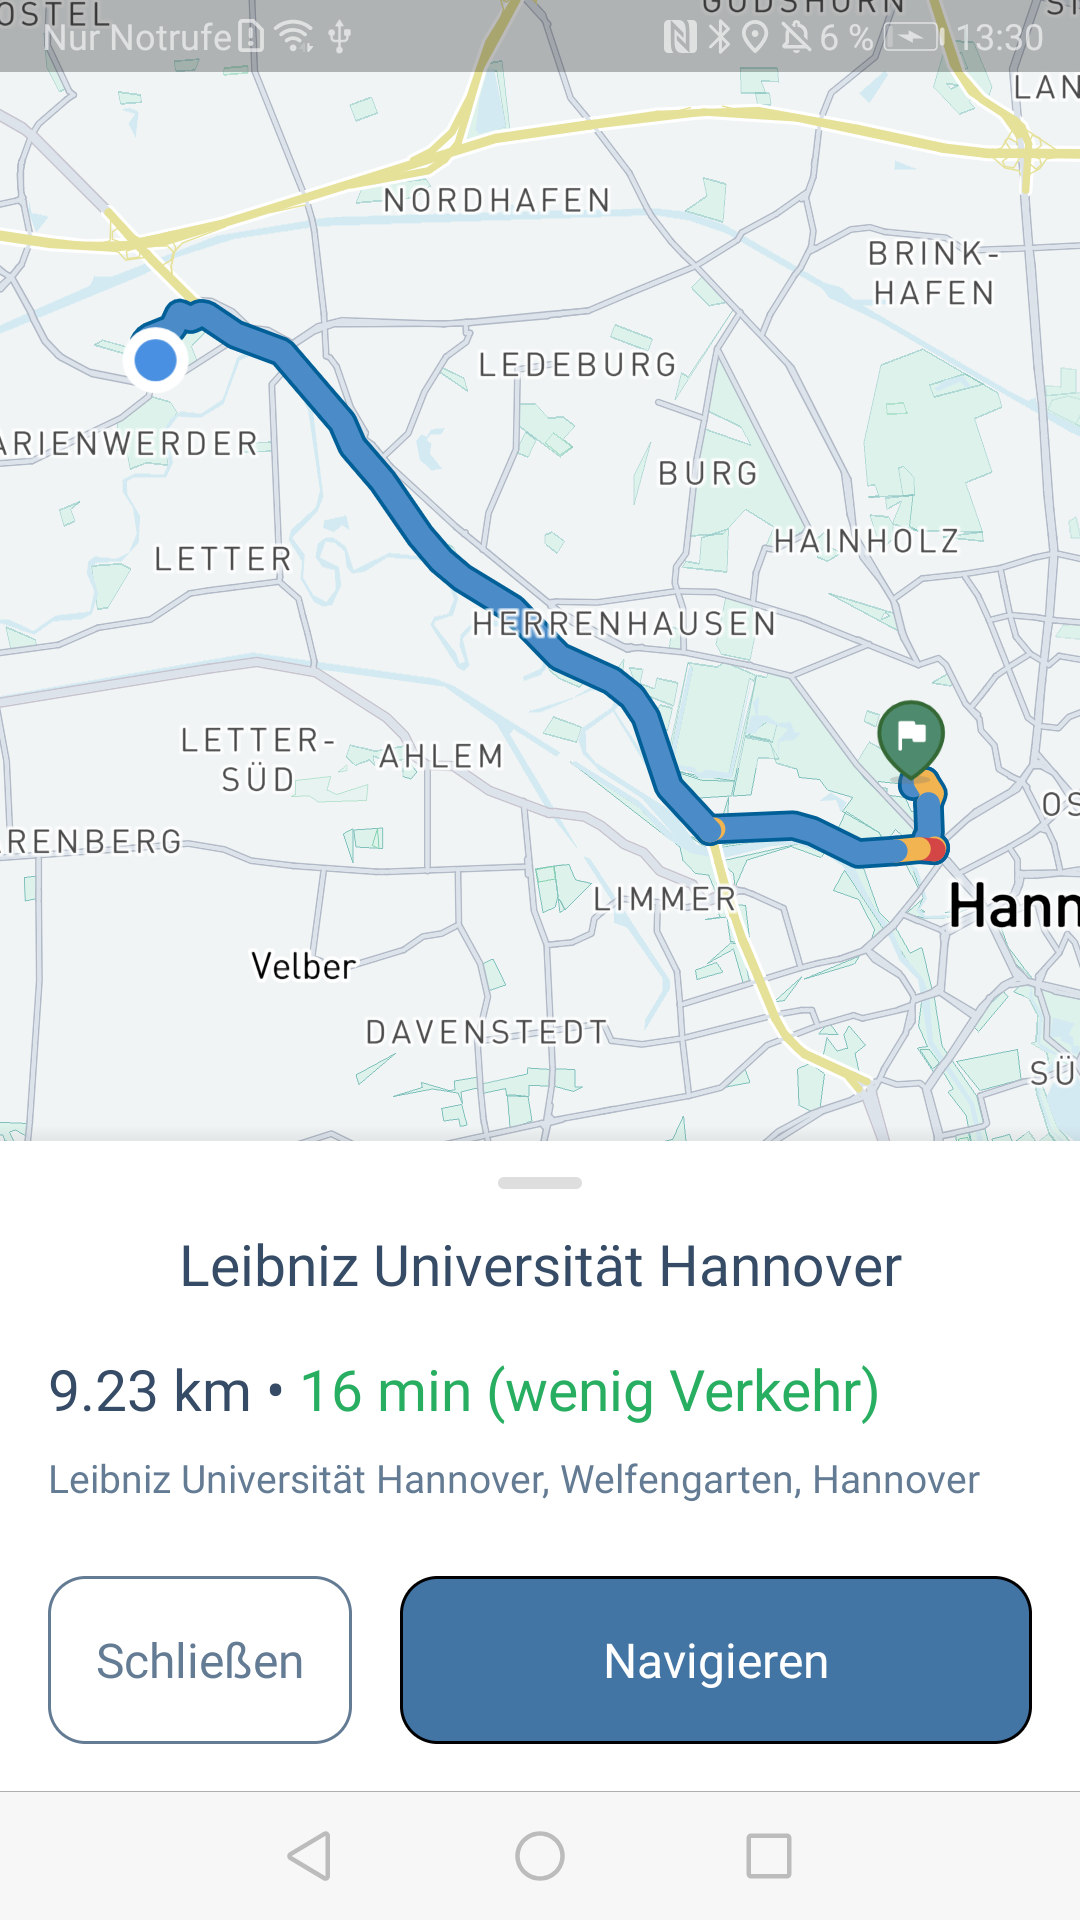
\includegraphics[width=.27\textwidth]{contents/06_model_evaluation/01_integration/res/03_traffic_volume/final_10.png}
    }
    \label{sec:appendix_traffic_volume_preview}
    \caption{Prototyp und finale Designs für die Erklärung zum aktuellen Verkehrsaufkommen in der Routenvorschau}
\end{figure}

\begin{figure}[htb!]
    \centering
    \subfloat[1. Prototyp zur Darstellung des aktuellen Verkehrsaufkommens]
    {
        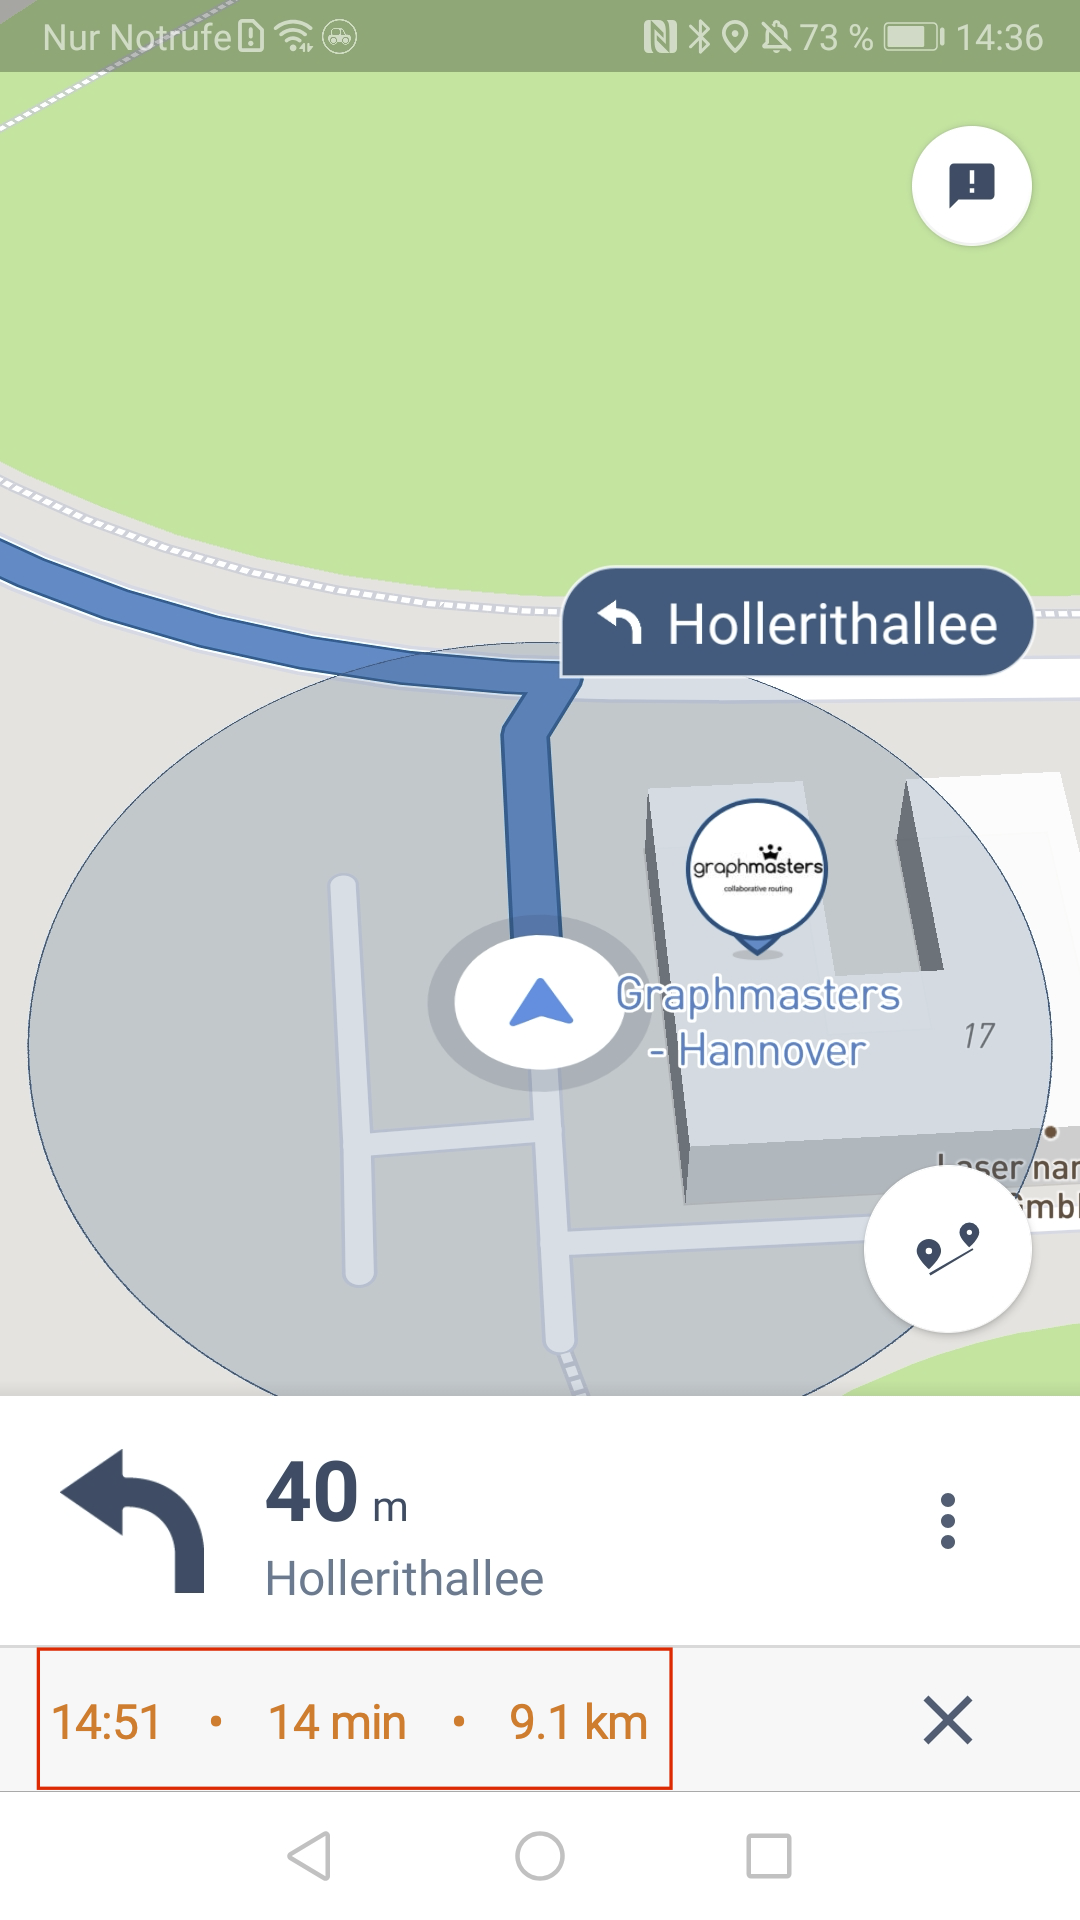
\includegraphics[width=.27\textwidth]{contents/06_model_evaluation/01_integration/res/03_traffic_volume/prototype_21.png}
    }
    \hspace{.055\textwidth}
    \subfloat[2. Prototyp zur Darstellung des aktuellen Verkehrsaufkommens]
    {
        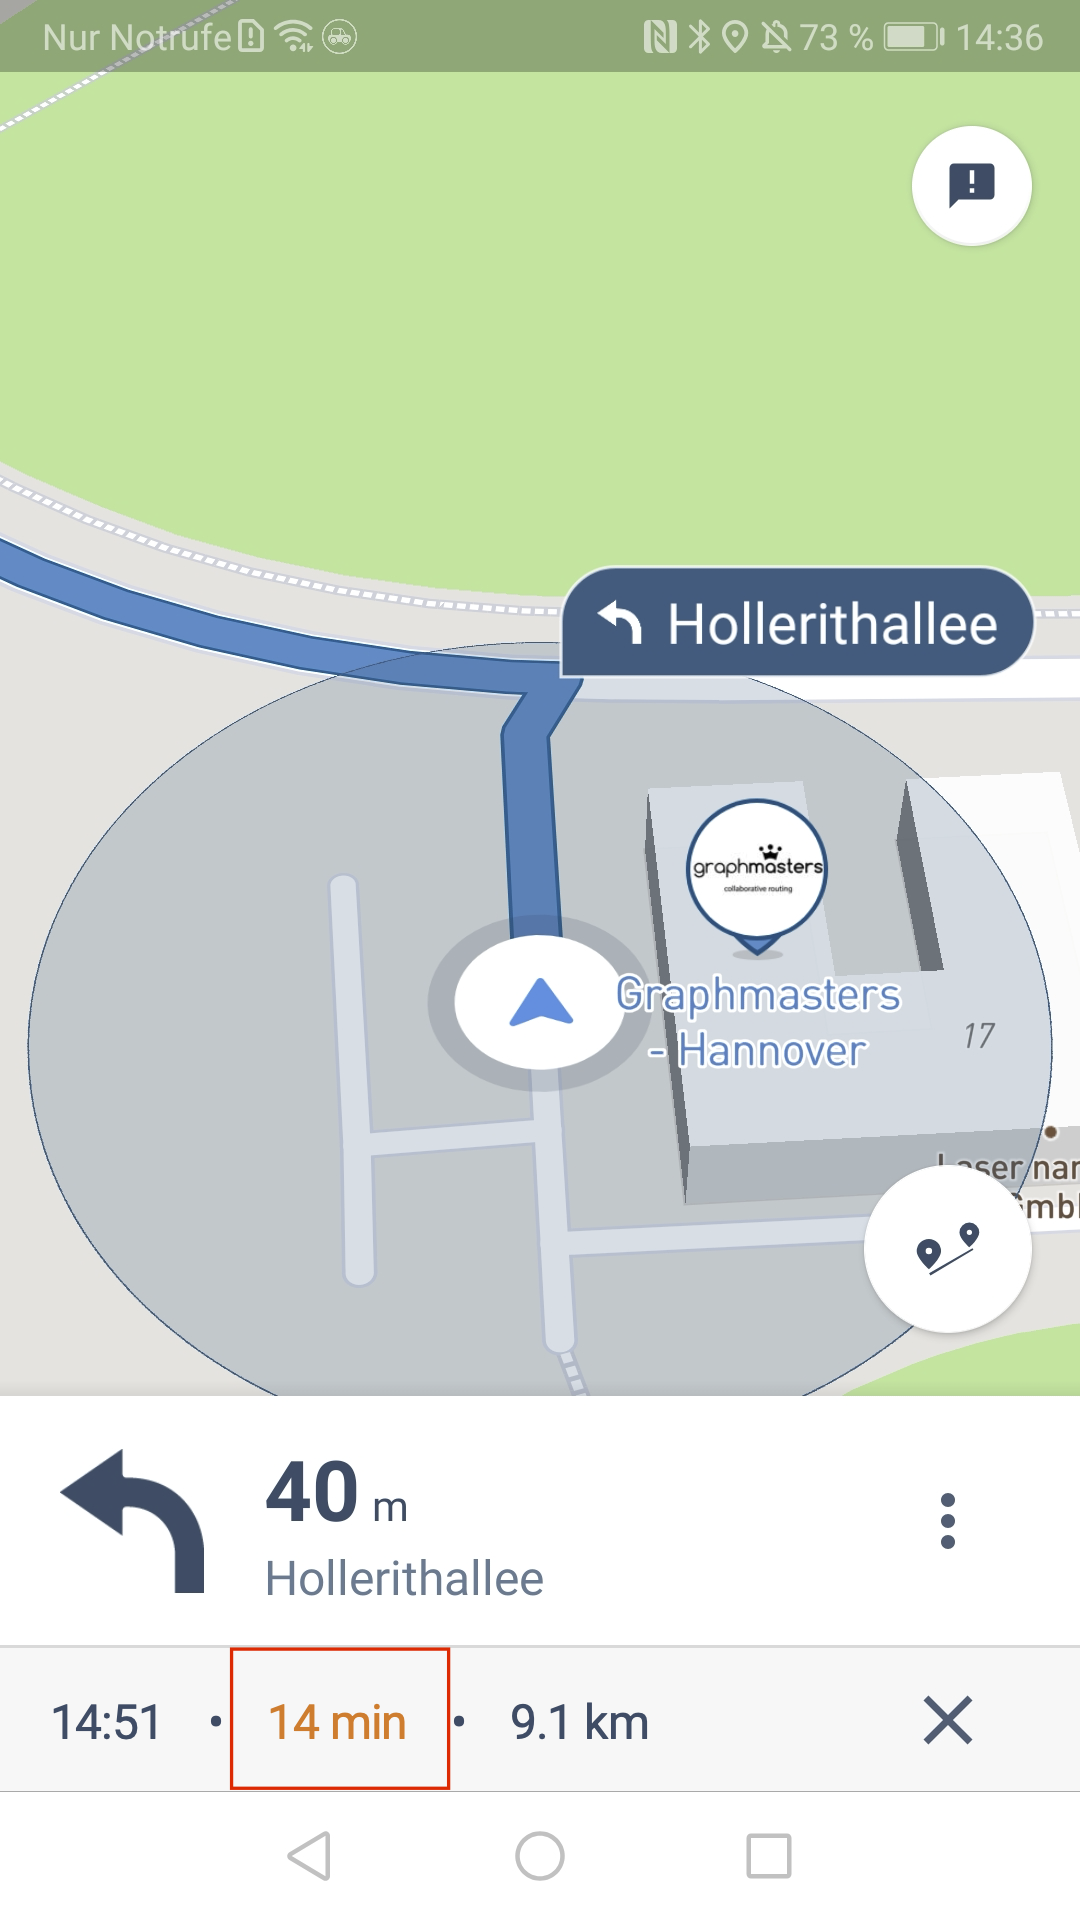
\includegraphics[width=.27\textwidth]{contents/06_model_evaluation/01_integration/res/03_traffic_volume/prototype_22.png}
    }
    \hspace{.055\textwidth}
    \subfloat[Finales Design zur Darstellung des aktuellen Verkehrsaufkommens]
    {
        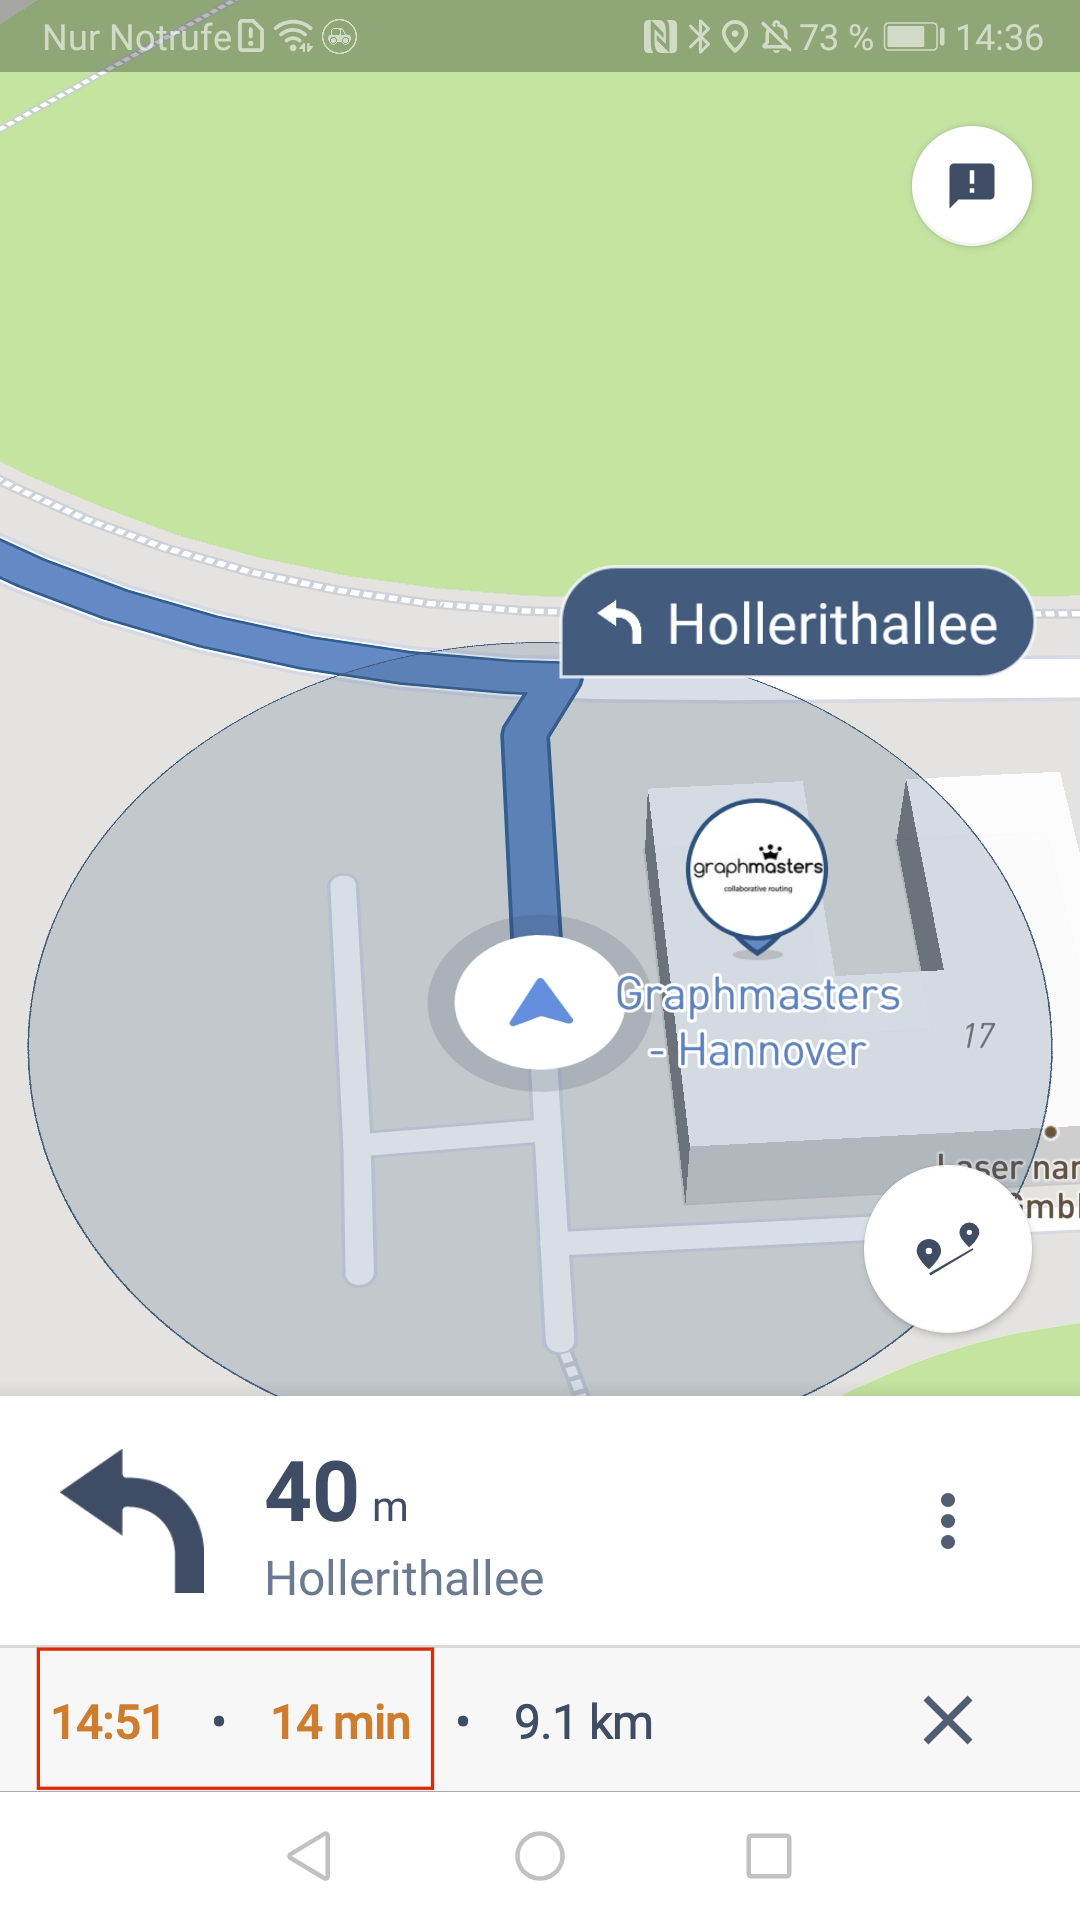
\includegraphics[width=.27\textwidth]{contents/06_model_evaluation/01_integration/res/03_traffic_volume/final_20.png}
    }
    \label{sec:appendix_traffic_volume_navigation}
    \caption{Prototyp und finale Designs für die Erklärung  zum aktuellen Verkehrsaufkommen während der Navigation}
\end{figure}

\newpage

\chapter{Evaluation der Erklärungen}

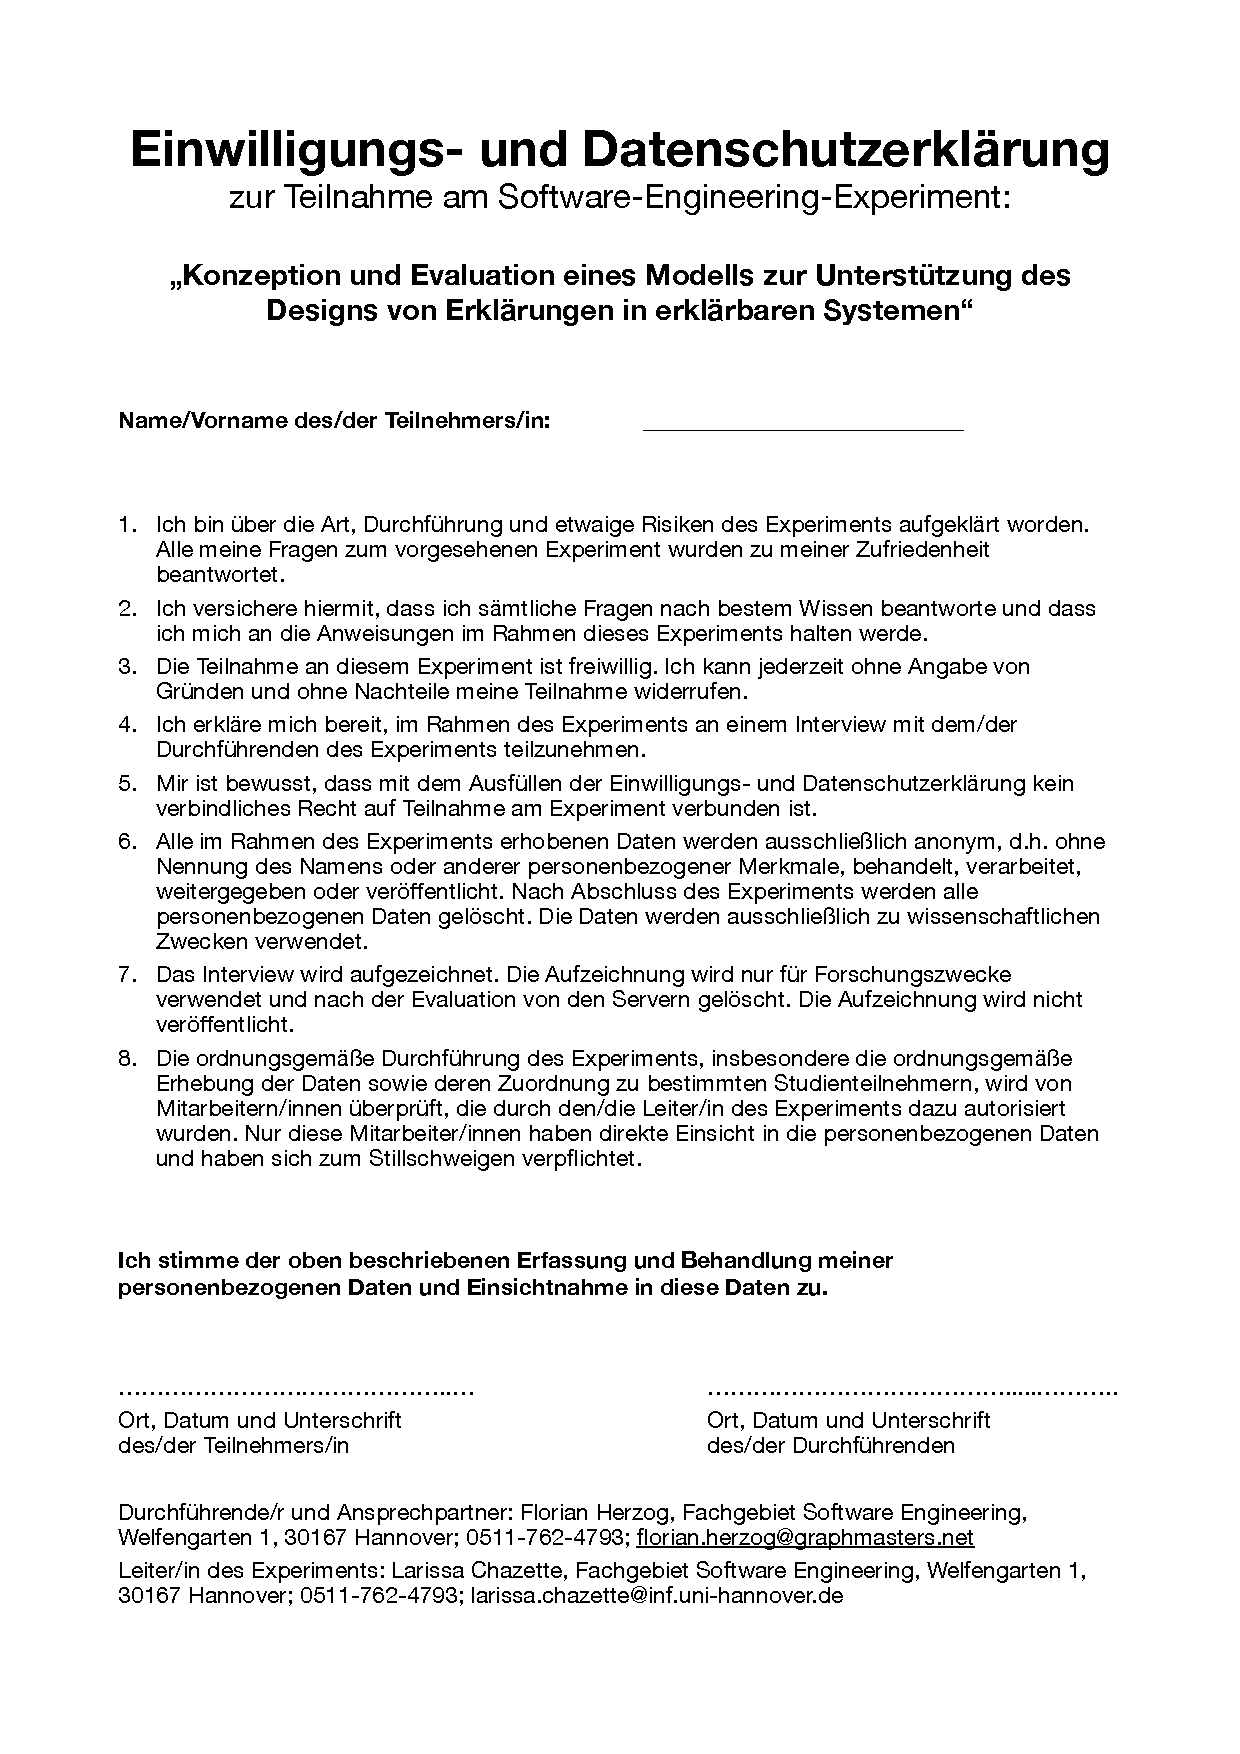
\includepdf[pages=1, scale=0.7,frame, pagecommand=\section*{Fragebogen des Quasi-Experiments}\label{sec:appendix_questionaire_protocol}]{contents/a_appendix/res/01_Questionaire_v3.pdf}
\includepdf[pages=2-, scale=0.7,frame]{contents/a_appendix/res/01_Questionaire_v3.pdf}